\documentclass[../../thesis.tex]{subfiles}

\graphicspath{{./img/}}

\begin{document}

    Our motivation in this analysis is that behind the transaction data stored on the Bitcoin Blockchain there is a hidden network which can provide valuable information on how agents made transactions through the usage of Bitcoins. As a consequence, we are interested in performing an analysis on the relationships between Bitcoin addresses. In this section, we introduce a way to translate the Bitcoin transactions into a Graph data structure which takes into consideration the time that the edge were created, and characterize this graph.

\section{Bitcoin as a Graph}
\label{sec:bitcoin_as_a_graph}


Our analysis begins by realizing that the Bitcoin transactions can be seen as a Graph. We saw in Section \ref{sec:bitcoin_transactions}, that a Bitcoin transaction is a record of input and output addresses. The addresses can be translated into the vertices of our Graph. The transferring of funds from \textit{Address A} to \textit{Address B} is converted to a directed edge from \textit{Address A} to \textit{Address B}. By design, the Bitcoin protocol allows a transaction to have more than one output address. Meaning, a user could transfer to more than one different user on the same transaction. Meaning, the relationship between inputs and outputs of a transaction is \textit{N to M}. For that reason, we can not discover from which input the funds are going exactly to which output. Figure \ref{fig:inputProblem}, visualizes this problem. Thus, we applied the same technique proposed on \cite{networkStructureBitcoin, richGetRicher}, where they state: 

\begin{quotation}
  A transaction with two inputs and three outputs results in six edges; an edge may appear multiple times, with the corresponding transaction.
\end{quotation}
In other words, we create an edge for all the possible combinations of inputs to outputs. Figure~\ref{fig:inputProblem} visualizes all the possible inputs and outputs pairs problem.


\begin{figure}
    \centering
    
    \begin{subfigure}{0.45\textwidth}
        \centering
        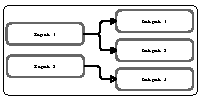
\includegraphics[width=0.9\textwidth]{content/unveiling/img/input-problem-1}         \caption{First possible combination.}
    \end{subfigure}\hfill
    \begin{subfigure}{0.45\textwidth}
        \centering
        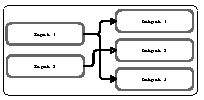
\includegraphics[width=0.9\textwidth]{content/unveiling/img/input-problem-2}         \caption{Second possible combination.}
    \end{subfigure}
    
     \begin{subfigure}{0.45\textwidth}
        \centering
        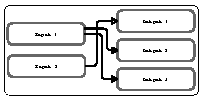
\includegraphics[width=0.9\textwidth]{content/unveiling/img/input-problem-3}         \caption{Third possible combination.}
    \end{subfigure}\hfill
    \begin{subfigure}{0.45\textwidth}
        \centering
        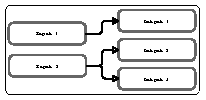
\includegraphics[width=0.9\textwidth]{content/unveiling/img/input-problem-4}         \caption{Fourth possible combination.}
    \end{subfigure}
    
     \begin{subfigure}{0.45\textwidth}
        \centering
        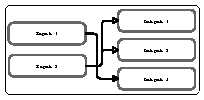
\includegraphics[width=0.9\textwidth]{content/unveiling/img/input-problem-5}         \caption{Fifth possible combination.}
    \end{subfigure}\hfill
    \begin{subfigure}{0.45\textwidth}
        \centering
        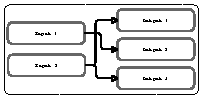
\includegraphics[width=0.9\textwidth]{content/unveiling/img/input-problem-6}        \caption{Sixth possible combination.}
    \end{subfigure}

\caption{Example of a transaction with two inputs and three outputs with all the possible arrangements of edges. By design, Bitcoin allows an edge to appear multiple times, within the corresponding transaction. Thus, we can not discover from which input the funds are going exactly to which output. }  
\label{fig:inputProblem}
\end{figure}



\begin{figure}
\centering

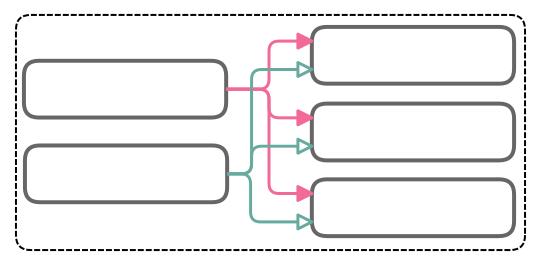
\includegraphics[width=\textwidth]{content/unveiling/img/input-solution}
\caption{The Solution of fig.\ref{fig:inputProblem}, a transaction with two inputs and three outputs results in six edges. We create an edge from each of the inputs to all of the outputs.}
\label{fig:inputSolution}
\end{figure}

However, Bitcoin users do not generate a static graph; the same address is allowed to make a transfer again in the future (if there are funds available). Consequently, the Bitcoin graph we are trying to create is not a simple graph, it is a graph that changes over time; one that evolves. Hence we must take into consideration the time. In our case, the time of the transaction that was broadcast on the network.

Hence, our final graph is a list of edges with timestamps. Note that we are not taking into consideration the amount of money transferred from one address to another, our sole interest is on the relationships between the vertices. 






\end{document}